% !TeX program = xelatex
\documentclass[10pt, a4paper]{article}

\usepackage{amsmath, amssymb, amsthm, mathtools}
\usepackage{geometry}
\usepackage{fancyhdr}
\usepackage{enumitem}
\usepackage{titlesec}
\usepackage{tocloft}
\usepackage[x11names]{xcolor}
\usepackage{graphicx}
\usepackage{float}
\usepackage{booktabs}
\usepackage{array}
\usepackage{multirow}
\usepackage{caption}
\usepackage{subcaption}
\usepackage{tikz}
\usepackage{microtype}
\usepackage{fontspec}
\usepackage{listings}
\newfontfamily\jpfont{Noto Sans CJK JP}
\usepackage[most]{tcolorbox}
\tcbuselibrary{skins, breakable}
\usepackage[backend=biber, citestyle=numeric-comp, bibstyle=numeric]{biblatex}
\usepackage{hyperref}
\usepackage{xurl}
\usepackage[capitalise, noabbrev]{cleveref}

\usetikzlibrary{arrows.meta, calc, positioning}

% --- Palette: Navy + Amber Gold ---
\definecolor{primary}{RGB}{28, 55, 90}
\definecolor{accent}{RGB}{176, 128, 52}
\definecolor{accentlight}{RGB}{232, 214, 178}
\definecolor{problembg}{RGB}{250, 248, 243}
\definecolor{problemframe}{RGB}{210, 220, 232}
\definecolor{textmuted}{RGB}{95, 105, 118}
\definecolor{coverbg}{RGB}{252, 249, 238}
\definecolor{progcolor}{RGB}{52, 105, 88}

% --- Page Geometry & Header/Footer ---
\geometry{left=2.4cm, right=2.4cm, top=2.6cm, bottom=2.6cm}
\setlength{\headheight}{18pt}
\setlength{\parindent}{1.5em}
\setlength{\parskip}{0.38em}
\linespread{1.15}
\emergencystretch=2em
\setlist{nosep, leftmargin=1.8em}

\pagestyle{fancy}
\fancyhf{}
\fancyhead[L]{\small\color{primary}\textsf{ADS Project 3: Recover the Design}}
\fancyhead[R]{\small\color{textmuted}\textsf{Fall--Winter 2026}}
\fancyfoot[C]{\small\color{textmuted}\thepage}
\renewcommand{\headrulewidth}{0.5pt}
\renewcommand{\headrule}{%
  {\color{accent!55}\hrule width\headwidth height 0.5pt}%
}

% --- Section & Subsection Headings ---
\titleformat{\section}
  {\color{primary}\centering\Large\bfseries}
  {\color{accent}Chapter~\thesection.}{0.6em}{}
  [\vspace{0.3em}{\color{accent!70}\titlerule[1.5pt]}]

\titleformat{name=\section,numberless}
  {\color{primary}\centering\Large\bfseries}
  {}{0pt}{}
  [\vspace{0.3em}{\color{accent!70}\titlerule[1.5pt]}]

\titleformat{\subsection}
  {\color{primary!88!black}\large\bfseries}
  {\color{accent}\thesubsection}{0.6em}{}
  [\vspace{0.15em}{\color{accent!45}\titlerule[0.8pt]}]

\titleformat{\subsubsection}
  {\color{primary!85!black}\normalsize\bfseries}
  {\color{accent}\thesubsubsection}{0.5em}{}

\titlespacing*{\section}{0pt}{0.6em}{1.0em}
\titlespacing*{\subsection}{0pt}{1.0em}{0.6em}
\titlespacing*{\subsubsection}{0pt}{0.8em}{0.4em}

% --- TOC Styling ---
\renewcommand{\cftsecfont}{\bfseries\color{primary}}
\renewcommand{\cftsecpagefont}{\bfseries\color{primary}}
\renewcommand{\cftsubsecfont}{\color{black!85}}
\renewcommand{\cftsubsubsecfont}{\small\color{textmuted}}
\setlength{\cftbeforesecskip}{0.55em}

% --- Styled Boxes ---
\newtcolorbox{insightbox}[1]{
    enhanced,
    breakable,
    colback=progcolor!5.5,
    colframe=progcolor!28,
    boxrule=0.7pt,
    arc=4pt,
    borderline west={3.5pt}{0pt}{progcolor},
    left=13pt,
    right=13pt,
    top=8pt,
    bottom=9pt,
    before skip=8pt plus 2pt,
    after skip=9pt plus 2pt,
    title={\sffamily #1},
    fonttitle=\bfseries,
    coltitle=white,
    colbacktitle=progcolor,
    attach boxed title to top left={yshift=-2mm, xshift=8mm},
    boxed title style={
        arc=2.5pt,
        boxrule=0pt,
        top=2pt,
        bottom=2pt,
        left=7pt,
        right=7pt,
    },
}

% --- Code Listings & Captions ---
\newcommand{\code}[1]{\texttt{\color{primary!90!black}#1}}
\newcommand{\kw}[1]{\textbf{\color{primary}#1}}
\newcommand{\id}[1]{\ensuremath{\mathrm{#1}}}
\captionsetup{labelfont={bf,color=primary}, skip=4pt}
\BeforeBeginEnvironment{tabular}{\small}

\lstset{
    language=C,
    basicstyle=\ttfamily\scriptsize,
    keywordstyle=\color{primary}\bfseries,
    commentstyle=\color{progcolor}\itshape,
    stringstyle=\color{accent},
    breaklines=true,
    numbers=left,
    numberstyle=\tiny\color{textmuted},
    frame=single,
    rulecolor=\color{problemframe},
    backgroundcolor=\color{problembg},
    captionpos=b,
    tabsize=4,
    columns=fullflexible,
    showstringspaces=false
}

\tikzset{
    conn/.style={circle, draw=primary, very thick, fill=primary!8, minimum size=7mm, inner sep=0pt, font=\footnotesize\bfseries, text=primary},
    fence/.style={line width=1.3pt, accent},
    cand/.style={line width=0.8pt, dashed, textmuted},
    bad/.style={line width=1.1pt, Red3}
}

\hypersetup{
    colorlinks=true,
    linkcolor=primary,
    citecolor=progcolor,
    urlcolor=accent,
    linktoc=all
}

\graphicspath{{../src/visualizations/}{../figure/}{image/}{figure/}}
\addbibresource[location=local]{reference.bib}

\begin{document}

% ============================================================
%  PAGE 1: DEDICATED COVER + ABSTRACT PAGE
% ============================================================
\begin{titlepage}
\begin{tikzpicture}[remember picture, overlay]
    \fill[coverbg] (current page.south west) rectangle (current page.north east);
    \draw[accent!40, line width=0.7pt]
        ([xshift=1.5cm, yshift=-1.5cm]current page.north west) --
        ([xshift=1.5cm, yshift=1.5cm]current page.south west);
    \draw[accent!40, line width=0.7pt]
        ([xshift=-1.5cm, yshift=-1.5cm]current page.north east) --
        ([xshift=-1.5cm, yshift=1.5cm]current page.south east);
    \foreach \r in {2.0, 2.45, 2.9} {
        \draw[primary!14, line width=0.5pt]
            ([xshift=-1.35cm, yshift=1.35cm]current page.south east) circle (\r cm);
        \draw[primary!14, line width=0.5pt]
            ([xshift=1.35cm, yshift=-1.35cm]current page.north west) circle (\r cm);
    }
\end{tikzpicture}

\vspace*{0.8cm}
\begin{center}
    {\large\color{accent}\textsf{\textbf{Advanced Data Structures and Algorithm Analysis}}}\\[0.25cm]
    {\normalsize\color{textmuted}\textsf{Laboratory Project Report $\cdot$ Project 3}}\\[0.6cm]

    {\color{primary}\rule{0.58\textwidth}{1.4pt}}\\[0.55cm]
    {\fontsize{23}{30}\selectfont\bfseries\color{primary} Recover the Design}\\[0.45cm]
    {\color{accent}\rule{0.24\textwidth}{1.0pt}}\\[0.55cm]
    {\Large\bfseries\color{accent}\textsf{Group X}}\\[0.7cm]

    {\Large\bfseries\color{primary} Student A \hspace{2.8em} Student B}\\[0.35cm]
    {\normalsize\color{textmuted}
        Zhejiang University \\[0.15cm]
        Date: 2026-11-02
    }
\end{center}

\vspace{0.8cm}
\begin{center}
    {\large\bfseries\color{primary} Abstract}
\end{center}
\vspace{-0.2em}
\begin{quote}
\small\noindent
In this project, we study \textbf{fence recovery} on an $n \times m$ grid, where straight horizontal and vertical fences must satisfy the target degree $k \in \{1,2,3,4\}$ of every connector without bending or intersecting at empty cells. We formulate the task as selecting a \textbf{degree-constrained subgraph} of \textbf{non-crossing edges} on a sparse \textbf{candidate graph}: each connector emits at most one rightward edge and one downward edge to its nearest visible neighbors, bounding the candidate set by $|E| \le 2|V|$. We then apply recursive \textbf{backtracking} with four \textbf{pruning} rules: a root handshaking parity check, a degree upper-bound check, a lookahead lower-bound check $\id{current}(v) + r(v,i) \ge d(v)$ over remaining incident edges, and an open-interval crossing check. We evaluate our solver on the three official samples, a scaling suite \code{L05}--\code{L20} and \code{U05}--\code{U20} from $5 \times 5$ to $20 \times 20$, and $360$ $100$-island instances on a $16 \times 16$ grid adapted from the \textbf{Hashiwokakero} benchmark into solvable single-fence boards. Every output on the solvable suites passes structural verification, and all odd-degree unsolvable boards are rejected in a single call. Across the $360$ benchmark instances where $|E| \in [168, 170]$, our solver explores a median of $\mathbf{931}$ \textbf{recursive calls} in $\mathbf{0.36\,\text{ms}}$ of pure search time and $53.90\,\text{ms}$ of end-to-end runtime. Finally, our analysis demonstrates the advantages of pruned backtracking: combining inclusion-first branching with lookahead degree bounds cuts infeasible subtrees early and keeps the actual search tree close to linear in $|E|$ despite the exponential worst case.

\vspace{0.55em}\noindent
{\color{primary}\textbf{Keywords:}} Fence recovery; degree-constrained subgraph; non-crossing edges; candidate graph; backtracking; pruning; Hashiwokakero.
\end{quote}

\vfill
\begin{center}
    {\color{accent!80}\rule{0.14\textwidth}{0.8pt}}\\[0.25cm]
    {\normalsize\bfseries\color{primary} Fall--Winter 2026}
\end{center}
\end{titlepage}

% ============================================================
%  PAGE 2: DEDICATED TABLE OF CONTENTS PAGE
% ============================================================
\pagenumbering{roman}
\thispagestyle{plain}
\vspace*{0.3cm}
\tableofcontents
\clearpage

% ============================================================
%  CHAPTER 1: INTRODUCTION
% ============================================================
\pagenumbering{arabic}
\section{Introduction}

\subsection{Problem Description}
In an $n \times m$ garden with $1 \le n, m \le 50$, some cells contain connectors of degree $1$ to $4$ and the rest are empty. The original fence drawing is lost; the task is to reconstruct straight horizontal and vertical fences that meet every connector's degree without bending or crossing in an empty cell, as illustrated in \Cref{fig:sample}. Given the degree matrix, the program outputs the four connection directions \texttt{up}, \texttt{down}, \texttt{left}, and \texttt{right} of each connector in row-major order, or \texttt{No Solution} if no valid layout exists.

This layout is closely related to the puzzle Hashiwokakero ({\jpfont 橋を架けろ}), where islands of given degrees are joined by non-crossing straight bridges~\cite{coelho2019hashi}. Unlike the classical puzzle, each direction here carries at most one fence and the fences need not form a single connected network. To solve this problem, we apply the backtracking method from the ADS course~\cite{ads_slides2026}:
\begin{itemize}
  \item \textbf{\color{primary}Backtracking:} Since every fence must end at the nearest visible connector in its row or column, all possible fences form a sparse candidate graph in which each edge is either selected or skipped. Depth-first search decides the candidate edges one by one and prunes a branch as soon as a connector exceeds its degree, lacks enough remaining edges to reach its degree, or introduces a crossing~\cite{ads_slides2026,weiss1996}.
\end{itemize}

\begin{figure}[H]
\centering
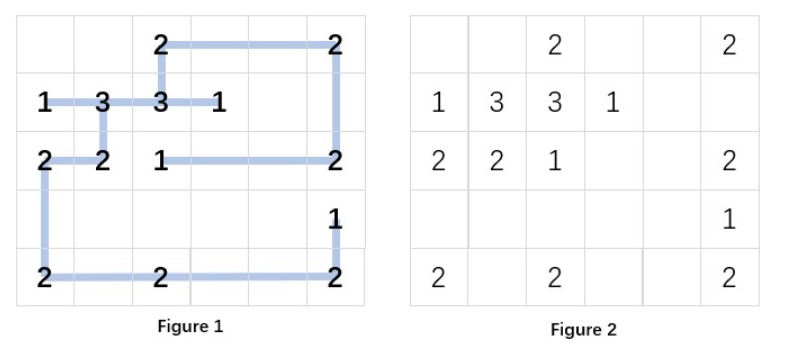
\includegraphics[width=0.92\textwidth]{figure1.png}
\caption{The assignment example.}
\label{fig:sample}
\end{figure}

\subsection{Purpose of This Report}
The goal of this project is to recover one feasible drawing by pruned backtracking and to measure that search on the boards we were given. Specifically, we:
\begin{enumerate}[label=\textbf{\color{primary}\arabic*.}]
  \item \textbf{Build the Candidate Graph and the Search:} Implement nearest-visible candidate fences and the pruned depth-first search in \code{recover\_the\_design.h} and \code{recover\_the\_design.c}.
  \item \textbf{Check Three Families of Boards:} Run the three official samples, the constructed boards \code{L05}--\code{L20} and \code{U05}--\code{U20}, and the $360$ revised $100$-island instances from the Coelho--Laporte--Lindbeck--Vidal benchmark~\cite{coelho2019hashi}.
  \item \textbf{Profile Scaling and Pruning Efficiency:} Measure recursive call counts and execution times across grid scales and analyze how lookahead pruning and degree slack govern search performance.
\end{enumerate}

\clearpage

% ============================================================
%  CHAPTER 2
% ============================================================
\section{Data Structure and Algorithm Specification}

\subsection{Overview of Board and Graph Representations}
\Cref{tab:structures} summarizes the core C data structures defined in \code{src/recover\_the\_design.h}. All grid cells are stored in a contiguous row-major array indexed by $\code{FlattenIndex}(x, y, m) = x \cdot m + y$. Empty cells remain in \code{vertices[]} with $\code{degree} = 0$, allowing row and column scans to check cell occupancy in $O(1)$ time without maintaining a separate grid matrix.

\begin{table}[H]
\centering
\caption{Summary of board and candidate-graph data structures implemented in \code{src/recover\_the\_design.h}.}
\label{tab:structures}
\begin{tabular}{@{}l>{\raggedright\arraybackslash}p{0.34\linewidth}>{\raggedright\arraybackslash}p{0.42\linewidth}@{}}
\toprule
\textbf{\color{primary}Structure} & \textbf{\color{primary}C Fields / Layout} & \textbf{\color{primary}Structural Invariant \& Role} \\
\midrule
\code{Vertex} & \code{int degree}, \code{int x}, \code{int y} & Represents one grid cell at 0-based coordinates $(x,y)$; $\code{degree} \in \{1,2,3,4\}$ denotes a connector and $\code{degree} = 0$ denotes an empty cell. \\
\code{Edge} & \code{Vertex from}, \code{Vertex to}, \code{int type}, \code{bool is\_selected} & Undirected candidate fence between two nearest visible connectors; \code{type} is \code{horizontal} or \code{vertical}, and \code{is\_selected} tracks whether the fence is active on the current search path. \\
\code{Graph} & \code{rows}, \code{columns}, \code{edge\_num}, \code{vertex\_num}, \code{int* current\_degree}, \code{Vertex* vertices}, \code{Edge* edges} & Holds the flattened cell array \code{vertices[]}, the candidate array \code{edges[]}, and the active degree counter \code{current\_degree[]} during backtracking. \\
\code{result} & \code{int x}, \code{int y}, \code{bool left}, \code{right}, \code{up}, \code{down} & Stores the four directional connection flags of each cell for row-major output formatting in \code{show\_result}. \\
\bottomrule
\end{tabular}
\end{table}

\subsection{Candidate Graph Construction}
Because a valid fence cannot bend or pass through an intermediate connector without terminating there, each connector only needs to be linked to its nearest visible connector in each of the four cardinal directions. Moreover, an undirected horizontal fence between $(x, y_1)$ and $(x, y_2)$ with $y_1 < y_2$ is shared by both endpoints, and the same holds for a vertical fence between $(x_1, y)$ and $(x_2, y)$ with $x_1 < x_2$. Consequently, \code{init\_Graph} scans the board in row-major order and emits at most two candidate edges from each connector: one to the nearest visible connector on its right, and one to the nearest visible connector below it.

\begin{table}[H]
\centering
\begin{tabular}{@{}p{1.6cm}p{0.81\textwidth}@{}}
\toprule
\multicolumn{2}{@{}l}{\textbf{\color{primary}Algorithm 1:} Candidate Graph Construction $\id{init\_Graph}(G, n, m)$ in \code{recover\_the\_design.h}} \\
\midrule
1. & Allocate $\code{vertices}[0..nm-1]$, $\code{current\_degree}[0..nm-1] \gets 0$, and $\code{edges}[0..4nm-1]$; read the $n \times m$ degree matrix into \code{vertices[]}. \\
2. & \kw{for each} cell $u = (x,y)$ in row-major order with $u.\id{degree} > 0$ \kw{do} \\
3. & \quad Advance $y' \gets y+1$ while $y' < m$ and $\code{vertices}[x \cdot m + y'].\id{degree} = 0$. \\
4. & \quad \kw{if} $y' < m$ \kw{then} append horizontal candidate edge $\bigl(u, (x, y')\bigr)$ to \code{edges[]} and increment \code{edge\_num}. \\
5. & \quad Advance $x' \gets x+1$ while $x' < n$ and $\code{vertices}[x' \cdot m + y].\id{degree} = 0$. \\
6. & \quad \kw{if} $x' < n$ \kw{then} append vertical candidate edge $\bigl(u, (x', y)\bigr)$ to \code{edges[]} and increment \code{edge\_num}. \\
\bottomrule
\end{tabular}
\end{table}

Since every connector contributes at most one rightward edge and one downward edge, the total number of candidate edges satisfies
\[
  |E| \;\le\; 2|V| \;\le\; 2nm.
\]
On the $100$-island benchmark boards, this bound is tight: every instance produces between $168$ and $170$ candidate edges.

\subsection{Backtracking Search and Pruning Rules}
Given the candidate array $\code{edges}[0..|E|-1]$, \code{backtrack} explores binary decisions from index $0$ to $|E|-1$, trying the inclusion branch $\code{is\_selected} = \code{true}$ before the exclusion branch $\code{is\_selected} = \code{false}$. Let $\id{current}(v)$ be the number of selected fences currently incident to $v$, and let $r(v, i)$ be the number of undecided candidate edges in $\code{edges}[i+1..|E|-1]$ incident to $v$, computed by \code{count\_remaining\_edges}. Four pruning rules cut infeasible branches before reaching a leaf:
\begin{itemize}
  \item \textbf{\color{primary}Handshaking Parity Check:} Every selected fence adds $2$ to the total degree across all connectors. At the root call $i = 0$, if $\sum_{v} d(v)$ is odd, \code{backtrack} immediately returns \code{false}~\cite{cormen2022}.
  \item \textbf{\color{primary}Degree Upper-Bound Check:} When edge $i = (u, w)$ is tentatively selected, \code{check\_edge} rejects the branch if $\id{current}(u) > d(u)$ or $\id{current}(w) > d(w)$.
  \item \textbf{\color{primary}Lookahead Lower-Bound Check:} A connector $v$ can still reach its target degree $d(v)$ only if
  \[
    \id{current}(v) + r(v, i) \;\ge\; d(v).
  \]
  This bound is enforced both inside \code{check\_edge} on the inclusion branch and in \code{backtrack} before entering the exclusion branch.
  \item \textbf{\color{primary}Orthogonal Crossing Check:} Two parallel edges never cross. A horizontal edge on row $x_h$ spanning columns $[y_1, y_2]$ and a vertical edge on column $y_v$ spanning rows $[x_1, x_2]$ cross at an empty interior cell if and only if
  \[
    y_1 < y_v < y_2 \quad\text{and}\quad x_1 < x_h < x_2.
  \]
  As shown in \Cref{fig:cross}, sharing a connector endpoint corresponds to equality at a boundary and is not treated as a crossing.
\end{itemize}

\begin{figure}[H]
\centering
\begin{tikzpicture}[x=1.0cm,y=0.92cm]
  \begin{scope}[xshift=0cm]
    \draw[step=1, color=problemframe, thin] (0,0) grid (3,2);
    \draw[bad] (0,1) -- (3,1);
    \draw[bad] (2,0) -- (2,2);
    \fill[Red3] (2,1) circle (2.2pt);
    \node[conn] at (0,1) {$A$};
    \node[conn] at (3,1) {$B$};
    \node[conn] at (2,2) {$C$};
    \node[conn] at (2,0) {$D$};
    \node[font=\footnotesize, anchor=north] at (1.5,-0.35) {(a) Illegal crossing};
  \end{scope}
  \begin{scope}[xshift=5.6cm]
    \draw[step=1, color=problemframe, thin] (0,0) grid (3,2);
    \draw[fence] (0,0) -- (2,0);
    \draw[fence] (2,0) -- (2,2);
    \node[conn] at (0,0) {$P$};
    \node[conn] at (2,0) {$Q$};
    \node[conn] at (2,2) {$R$};
    \node[font=\footnotesize, anchor=north] at (1.5,-0.35) {(b) Legal corner at $Q$};
  \end{scope}
\end{tikzpicture}
\caption{\footnotesize Crossing check.}
\label{fig:cross}
\end{figure}

\begin{table}[H]
\centering
\begin{tabular}{@{}p{2.1cm}p{0.77\textwidth}@{}}
\toprule
\multicolumn{2}{@{}l}{\textbf{\color{primary}Algorithm 2:} Recursive Search $\id{Backtrack}(G, i)$ and $\id{check\_edge}(G, i)$} \\
\midrule
\textbf{Backtrack:} &
1. \kw{if} $i = 0$ and $\sum_v d(v)$ is odd \kw{then return} \code{false}. \\
& 2. \kw{if} $i = |E|$ \kw{then return} $\code{true}$ if $\id{current}(v) = d(v)$ for all $v$, else \code{false}. \\
& 3. Set $\code{edges}[i].\id{is\_selected} \gets \code{true}$ and increment $\id{current}(u), \id{current}(w)$ for endpoints $u, w$. \\
& 4. \kw{if} $\id{check\_edge}(G, i)$ and $\id{Backtrack}(G, i+1)$ \kw{then return} \code{true}. \\
& 5. Set $\code{edges}[i].\id{is\_selected} \gets \code{false}$ and decrement $\id{current}(u), \id{current}(w)$. \\
& 6. \kw{if} $\id{current}(u) + r(u,i) \ge d(u)$ and $\id{current}(w) + r(w,i) \ge d(w)$ \kw{and} $\id{Backtrack}(G, i+1)$ \kw{then return} \code{true}. \\
& 7. \kw{return} \code{false}. \\[0.25em]
\textbf{Check-Edge:} &
1. \kw{if} $\id{current}(u) > d(u)$ or $\id{current}(w) > d(w)$ \kw{then return} \code{false}. \\
& 2. \kw{if} $\id{current}(u) + r(u,i) < d(u)$ or $\id{current}(w) + r(w,i) < d(w)$ \kw{then return} \code{false}. \\
& 3. \kw{for} $j = 0$ \kw{to} $|E|-1$ \kw{do if} $\code{edges}[j].\id{is\_selected}$ and $\id{is\_crossing}(\code{edges}[j], \code{edges}[i])$ \kw{then return} \code{false}. \\
& 4. \kw{return} \code{true}. \\
\bottomrule
\end{tabular}
\end{table}

\subsection{Directional Output Formatting}
Once \code{backtrack} returns \code{true}, \code{show\_result} allocates a zero-initialized array $\code{res}[0..nm-1]$ of \code{result} records. Each selected horizontal edge sets $\code{right} = \code{true}$ on its left endpoint and $\code{left} = \code{true}$ on its right endpoint; each selected vertical edge sets $\code{down} = \code{true}$ on its upper endpoint and $\code{up} = \code{true}$ on its lower endpoint. Scanning the grid in row-major order and skipping empty cells prints each connector in the required 1-based format \texttt{row col up down left right}.

\clearpage

% ============================================================
%  CHAPTER 3: TESTING RESULTS
% ============================================================
\section{Testing Results}

\subsection{Dataset Links and Benchmark Specifications}
We evaluate our solver on three groups of puzzle boards:
\begin{itemize}
  \item \textbf{Official Problem Samples:} Three small test cases from the problem specification: a solvable $5 \times 6$ board shown in \Cref{fig:sample}, an unsolvable $5 \times 6$ board with an odd degree sum, and a $3 \times 5$ board that admits two distinct valid drawings.
  \item \textbf{Constructed Scaling Suite, \code{recover\_the\_design\_large\_tests.txt}:} Sixteen solvable $n \times n$ boards \code{L05}--\code{L20} with $n \in [5, 20]$, together with four unsolvable odd-degree boards \code{U05}, \code{U10}, \code{U15}, and \code{U20}.
  \item \textbf{Revised 100-Island Hashiwokakero Benchmark:} Obtained from the public benchmark of Coelho et al.~\cite{coelho2019hashi} at \url{https://w1.cirrelt.ca/~vidalt/en/research-data.html}, which provides $360$ $100$-island instances on a $16 \times 16$ grid. Because the original puzzles allow double bridges and island degrees up to $8$, we modified them into solvable single-fence instances under \code{data/Hashi\_Puzzles/100\_revised/} by keeping all $100$ island positions fixed, removing the island-count header token, and adjusting positive degrees into $\{1,2,3,4\}$ from a valid non-crossing single-fence layout stored in \code{100\_solutions/}.
\end{itemize}

\subsection{Test Suite and Structural Verification}
Because a degree matrix can admit multiple valid fence layouts, our checker \code{verify\_output.py} validates the output against the four layout rules rather than requiring byte-identical text: every connector must appear once in row-major order, the four directional flags at each connector must sum to its required degree, every active direction must match the opposite flag on the nearest visible connector across empty cells, and no horizontal fence may cross a vertical fence. \Cref{tab:testcases} summarizes all test cases.

\vspace{-0.2em}
\begin{table}[H]
\centering
\caption{Summary of functional, structural, and large-scale performance test cases.}
\label{tab:testcases}
\renewcommand{\arraystretch}{1.05}
\setlength{\tabcolsep}{3.2pt}
\footnotesize
\begin{tabular}{@{}c
  >{\raggedright\arraybackslash}p{0.21\linewidth}
  >{\raggedright\arraybackslash}p{0.26\linewidth}
  >{\raggedright\arraybackslash}p{0.31\linewidth}
  c@{}}
\toprule
\textbf{\color{primary}ID} & \textbf{\color{primary}Test Purpose} & \textbf{\color{primary}Expected Result} & \textbf{\color{primary}Actual Behavior} & \textbf{\color{primary}Status} \\
\midrule
TC-1 & Official $5 \times 6$ Sample~1 in \Cref{fig:sample} & Valid 14-line connector layout matching Sample Output~1 & Output matches Sample Output~1 byte for byte; $13$ fences, $19$ calls & Pass \\
TC-2 & Official $5 \times 6$ Sample~2 with cell $(3,6)$ lowered to $1$ & \texttt{No Solution} & Odd degree sum $25$ rejected at root in $1$ call & Pass \\
TC-3 & Official $3 \times 5$ Sample~3 with multiple valid layouts & Either of the two valid 8-fence drawings & Returns Sample Output~3 in $16$ calls; verified by \code{verify\_output.py} & Pass \\
TC-4 & Solvable scaling suite \code{L05}--\code{L20}, $5 \times 5$ to $20 \times 20$ & All degree, visibility, and non-crossing rules hold & All $16$ boards pass verification; $|V|$ grows from $21$ to $280$ and $|E|$ from $32$ to $520$ & Pass \\
TC-5 & Unsolvable boards \code{U05}, \code{U10}, \code{U15}, and \code{U20} & \texttt{No Solution} & Odd degree sums $51$, $171$, $379$, and $755$ each rejected in $1$ call & Pass \\
TC-6 & Structural verification on $360$ revised $100$-island boards & Valid layout for every \code{.has} instance & All $360$ outputs pass \code{verify\_output.py}; median $931$ calls & Pass \\
TC-7 & Batch runtime logging via \code{testbench\_time.c} & Complete CSV log without timeout & All $360$ runtimes logged in \code{benchmark\_results\_100.csv}; median $53.90\,\text{ms}$, max $189.88\,\text{ms}$ & Pass \\
\bottomrule
\end{tabular}
\end{table}
\vspace{-0.3em}

In TC-2, lowering the connector at $(3,6)$ from $2$ to $1$ changes the total degree from $26$ to $25$, so the root parity check in \code{backtrack} rejects the board before testing any candidate edge. In TC-3, the $3 \times 5$ board has exactly two valid drawings of eight fences, which differ in whether the degree-$1$ connector at $(1,1)$ connects rightward to $(1,2)$ or downward to $(2,1)$. Because \code{init\_Graph} emits the rightward edge first and \code{backtrack} tries inclusion before exclusion, our solver outputs the rightward layout matching Sample Output~3.

\subsection{Performance Benchmark Setup and Runtime Tables}
To evaluate both algorithmic search cost and end-to-end execution time, we record two sets of measurements:
\begin{itemize}
  \item \textbf{Pure Backtracking Search Profile:} Compiled with \texttt{gcc -O2}, \code{testbench\_profile.c} instruments \code{backtrack} to record the number of candidate edges $|E|$, selected fences $|E^*|$, recursive calls, and in-memory search time excluding process creation and file I/O.
  \item \textbf{End-to-End Batch Timing:} On Windows, \code{testbench\_time.c} spawns \code{recover\_the\_design.exe} once per \code{.has} file with a $60\,\text{s}$ timeout and measures wall-clock time via \code{QueryPerformanceCounter}, writing all $360$ records to \code{benchmark\_results\_100.csv}.
\end{itemize}

\vspace{-0.2em}
\begin{table}[H]
\centering
\caption{Backtracking search profile on the constructed boards \code{L05}--\code{L20}.}
\label{tab:large}
\renewcommand{\arraystretch}{0.92}
\setlength{\tabcolsep}{4.4pt}
\begin{tabular}{@{}lrrrrrr@{}}
\toprule
\textbf{\color{primary}Board} & \textbf{\color{primary}Grid} & \textbf{\color{primary}Connectors $|V|$} & \textbf{\color{primary}Candidates $|E|$} & \textbf{\color{primary}Selected $|E^*|$} & \textbf{\color{primary}Calls} & \textbf{\color{primary}Search Time, ms} \\
\midrule
\code{L05} & $5 \times 5$   &  21 &  32 &  25 &      37 & 0.015 \\
\code{L08} & $8 \times 8$   &  38 &  60 &  43 &      66 & 0.020 \\
\code{L10} & $10 \times 10$ &  67 & 114 &  85 &     197 & 0.153 \\
\code{L12} & $12 \times 12$ & 101 & 178 & 126 &     536 & 0.254 \\
\code{L14} & $14 \times 14$ & 140 & 252 & 187 &     430 & 0.244 \\
\code{L16} & $16 \times 16$ & 177 & 322 & 239 &     754 & 0.536 \\
\code{L18} & $18 \times 18$ & 229 & 422 & 304 & $8{,}544$ & 8.340 \\
\code{L20} & $20 \times 20$ & 280 & 520 & 377 & $1{,}238$ & 1.360 \\
\bottomrule
\end{tabular}
\end{table}
\vspace{-0.3em}

\vspace{-0.2em}
\begin{table}[H]
\centering
\caption{Distribution summary of structural and runtime metrics across the $360$ revised $100$-island benchmark instances on a $16 \times 16$ grid.}
\label{tab:groups}
\renewcommand{\arraystretch}{0.95}
\setlength{\tabcolsep}{4.8pt}
\begin{tabular}{@{}lrrrrrrr@{}}
\toprule
\textbf{\color{primary}Metric} & \textbf{\color{primary}Min} & \textbf{\color{primary}25th Pct} & \textbf{\color{primary}Median} & \textbf{\color{primary}Mean} & \textbf{\color{primary}SD} & \textbf{\color{primary}95th Pct} & \textbf{\color{primary}Max} \\
\midrule
Candidate Edges $|E|$          & 168.00 & 168.00 & 168.00 &   168.23 &     0.48 &    169.00 &     170.00 \\
Selected Fences $|E^*|$        &  75.00 &  87.00 &  91.00 &    91.23 &     5.83 &    101.00 &     105.00 \\
Recursive Calls $T$            & 172.00 & 375.75 & 930.50 & 3{,}455.28 & 9{,}580.19 & 13{,}312.30 & 110{,}997.00 \\
Pure Search Time, ms           &   0.08 &   0.16 &   0.36 &     1.22 &     3.17 &      4.44 &      30.51 \\
End-to-End Runtime, ms         &  41.71 &  49.45 &  53.90 &    59.40 &    17.73 &     91.63 &     189.88 \\
\bottomrule
\end{tabular}
\end{table}
\vspace{-0.3em}

\subsection{Runtime Plots and Recovered Fence Layouts}
\Cref{fig:scaling,fig:overview,fig:showcase} present the benchmark plots and recovered fence layouts generated by \code{visualization.py}. On the constructed boards \code{L05}--\code{L20} in \Cref{fig:scaling}, $|V|$, $|E|$, and $|E^*|$ grow smoothly with grid width $n$, and most boards finish within $200\text{--}1{,}400$ recursive calls and under $1.4\,\text{ms}$, except for \code{L18} which explores $8{,}544$ calls in $8.34\,\text{ms}$ before finding a valid layout.

Across the $360$ revised $100$-island instances in \Cref{fig:overview}, every board has $168\text{--}170$ candidate edges; pure search time has a median of $0.36\,\text{ms}$, a mean of $1.22\,\text{ms}$, and a maximum of $30.51\,\text{ms}$ at $110{,}997$ calls, whereas end-to-end process runtime has a minimum of $41.71\,\text{ms}$, a median of $53.90\,\text{ms}$, a mean of $59.40\,\text{ms}$, a $95\text{th}$ percentile of $91.63\,\text{ms}$, and a maximum of $189.88\,\text{ms}$. Finally, \Cref{fig:showcase} visualizes the non-crossing fence layouts recovered by our solver on three representative boards: \code{L08} ($8 \times 8$), \code{L12} ($12 \times 12$), and Benchmark Instance~\#1 (\code{Hs\_16\_100\_25\_00\_001.has}, $16 \times 16$), where solid amber segments denote selected fences and dashed gray segments denote unselected candidate edges.

\vspace{-0.2em}
\begin{figure}[H]
\centering
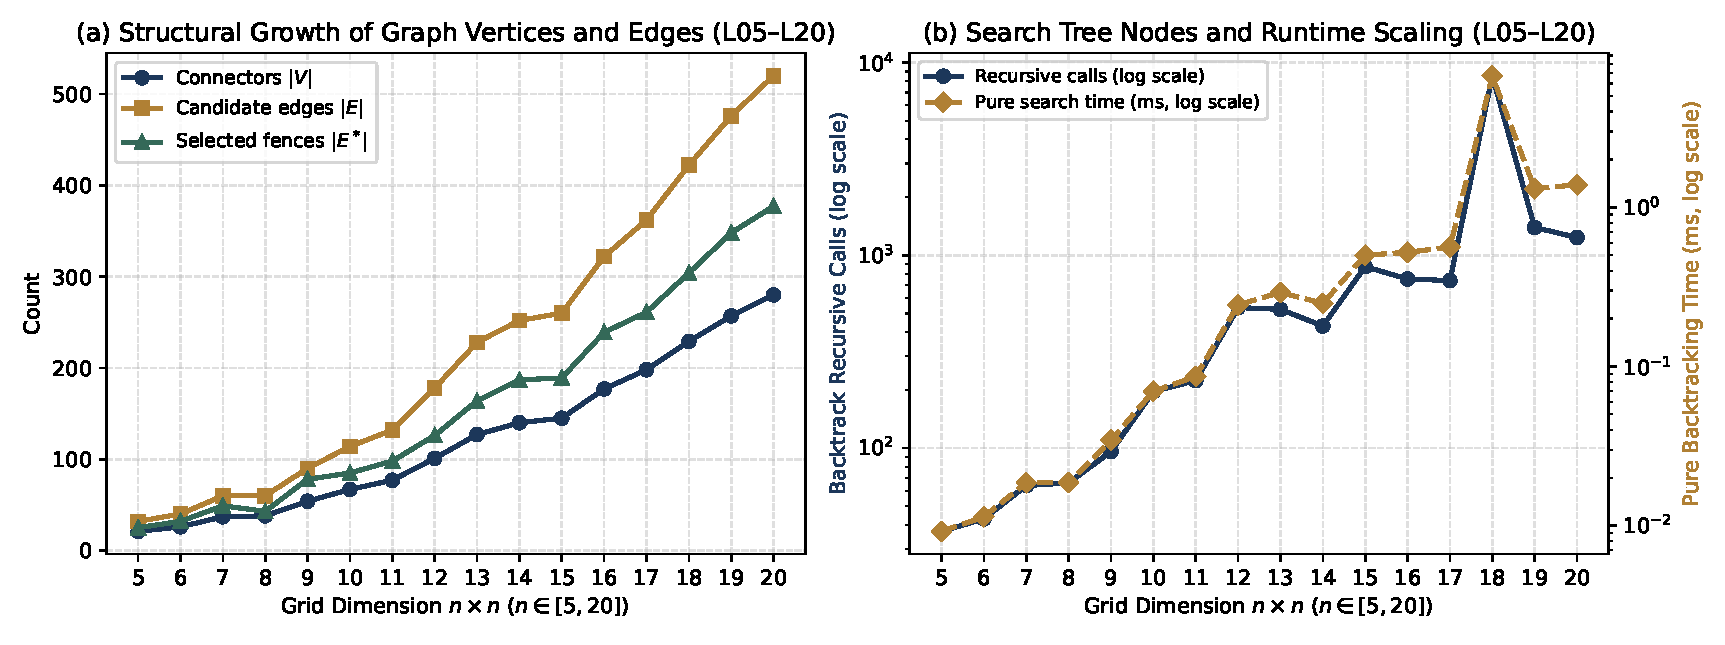
\includegraphics[width=0.96\textwidth]{large_tests_scaling.pdf}
\caption{\footnotesize Structural growth and search scaling on \code{L05}--\code{L20}.}
\label{fig:scaling}
\end{figure}

\vspace{-0.2em}
\begin{figure}[H]
\centering
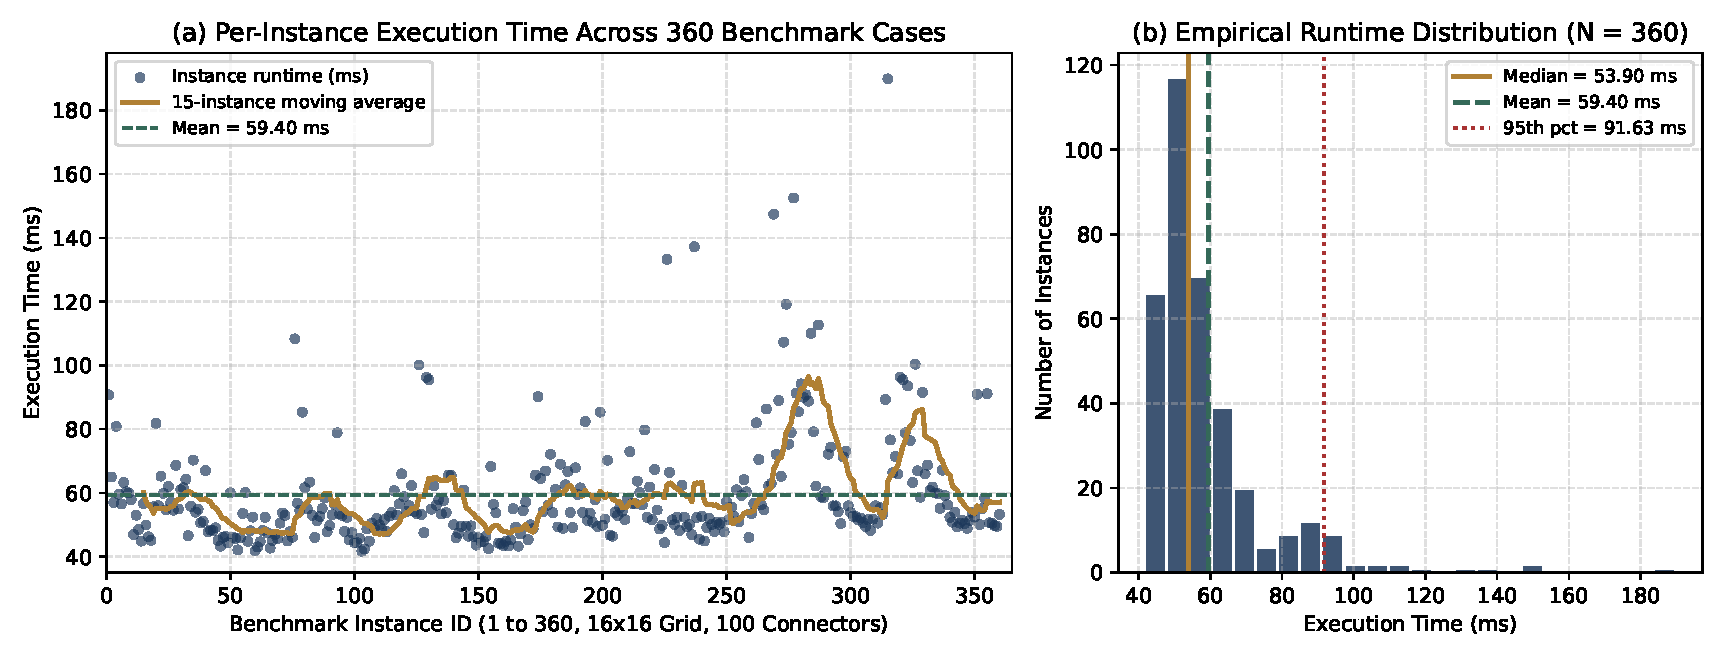
\includegraphics[width=0.96\textwidth]{hashi100_runtime_overview.pdf}
\caption{\footnotesize End-to-end execution time across the $360$ revised $100$-island benchmark instances.}
\label{fig:overview}
\end{figure}

\vspace{-0.2em}
\begin{figure}[H]
\centering
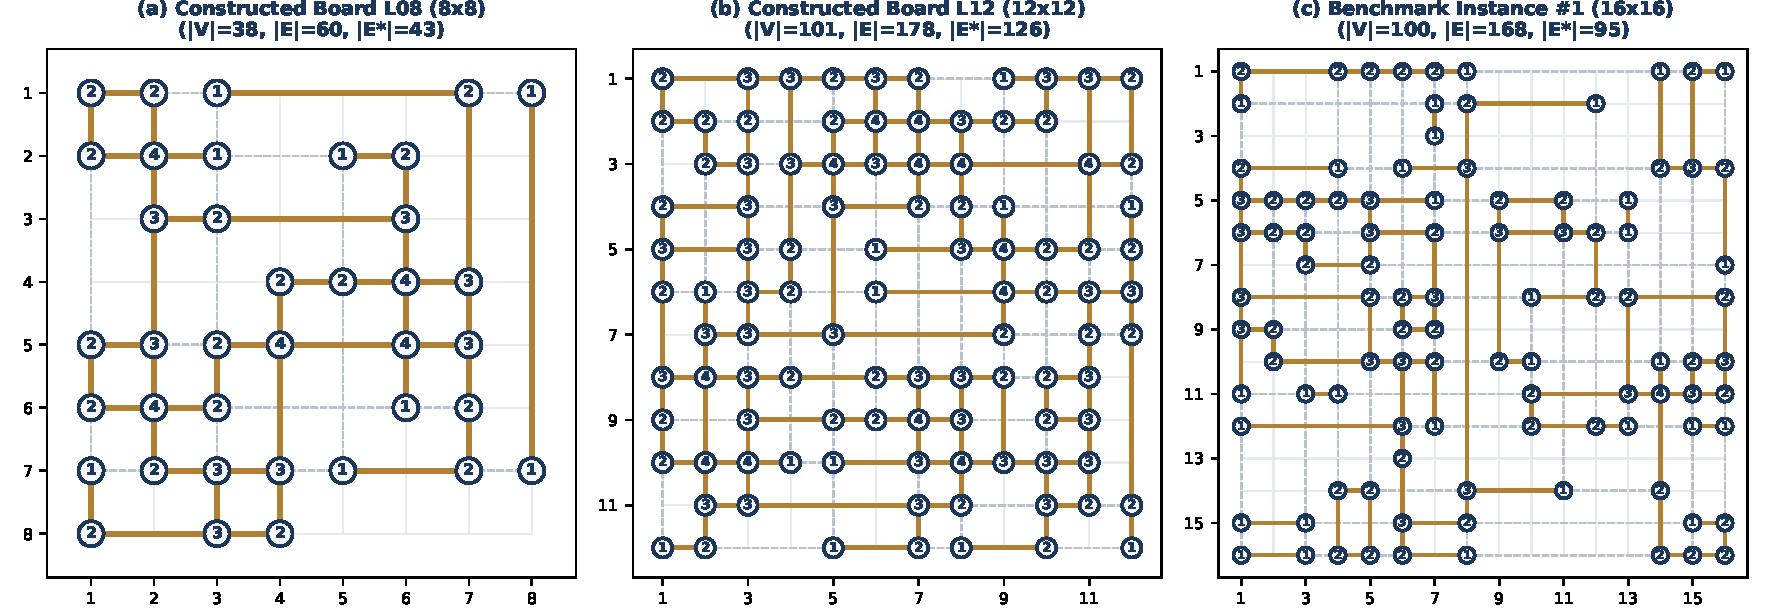
\includegraphics[width=0.96\textwidth]{recovered_layouts_showcase.pdf}
\caption{\footnotesize Recovered fence layouts on \code{L08}, \code{L12}, and Benchmark Instance~\#1.}
\label{fig:showcase}
\end{figure}

\clearpage

% ============================================================
%  CHAPTER 4: ANALYSIS AND COMMENTS
% ============================================================
\section{Analysis and Comments}

\subsection{Time and Space Complexity Analysis}
Let $T$ be the number of recursive calls to \code{backtrack} before the search terminates. \Cref{tab:complexities} summarizes the theoretical time and space complexities of each stage of our solver on an $n \times m$ board with $|V|$ connectors and $|E|$ candidate fences.

\begin{table}[H]
\centering
\caption{Theoretical time and space complexities of candidate-graph construction and pruned backtracking.}
\label{tab:complexities}
\setlength{\tabcolsep}{4.0pt}
\begin{tabular}{@{}lccc@{}}
\toprule
\textbf{\color{primary}Stage / Operation} & \textbf{\color{primary}Count per Instance} & \textbf{\color{primary}Time Complexity} & \textbf{\color{primary}Auxiliary Space} \\
\midrule
Grid \& Candidate Init (\code{init\_Graph}) & $1$ & $\Theta(nm)$ & $\Theta(nm)$ \\
Root Parity Check & $1$ & $\Theta(nm)$ & $\Theta(1)$ \\
Lookahead \& Crossing Check (\code{check\_edge}) & $\le T$ & $O(|E|)$ & $\Theta(1)$ \\
Leaf Verification ($i = |E|$) & $\le T$ & $\Theta(nm)$ & $\Theta(1)$ \\
Output Formatting (\code{show\_result}) & $1$ & $\Theta(nm + |E|)$ & $\Theta(nm)$ \\
\midrule
\textbf{Unpruned Search Tree} & $2^{|E|+1}-1$ nodes & $O(|E|\cdot 2^{|E|})$ & $\Theta(nm + |E|)$ \\
\textbf{Pruned Backtracking Search} & $T \le 2^{|E|+1}-1$ & $O(|E|\cdot T + nm)$ & $\Theta(nm + |E|)$ \\
\bottomrule
\end{tabular}
\end{table}

\noindent\textbf{Time Complexity Details.} In \code{init\_Graph}, reading the $n \times m$ grid takes $\Theta(nm)$ time, and scanning rightward and downward from each connector visits only empty cells before stopping at the first visible neighbor, so each empty cell is traversed at most once horizontally and once vertically, totaling $\Theta(nm)$ time. Inside each recursive call at index $i$, \code{count\_remaining\_edges} scans the suffix $\code{edges}[i+1..|E|-1]$ for both endpoints in $O(|E|)$ time, and \code{check\_edge} scans $\code{edges}[0..|E|-1]$ to test crossings in $O(|E|)$ time. Because $|E| \le 2|V| \le 2nm$, the worst-case unpruned search takes $O(|E|\cdot 2^{|E|})$ time, whereas our pruned search takes $O(|E|\cdot T + nm)$ time.

\paragraph{Space Complexity Details.}
\code{init\_Graph} allocates $\code{vertices}[0..nm-1]$, $\code{current\_degree}[0..nm-1]$, and $\code{edges}[0..4nm-1]$, while \code{show\_result} allocates $\code{res}[0..nm-1]$; all four arrays take $\Theta(nm)$ space. During recursion, the call stack reaches depth at most $|E| + 1 \le 2|V| + 1$ with $O(1)$ local variables per frame, so total auxiliary space is $\Theta(nm + |E|) = \Theta(nm)$.

\subsection{Why Pruned Backtracking Performs Well on Benchmark Instances}
Two empirical findings from Chapter~3 explain both the speed of the recursion and the variance across individual boards.

\vspace{-0.3em}
\begin{insightbox}{Key Finding 1: Inclusion-First Ordering and Lookahead Pruning Keep $T$ Near $|E|$}
Trying the inclusion branch before the exclusion branch constructs a valid layout from the earliest feasible candidates, while the lookahead bound $\id{current}(v) + r(v,i) \ge d(v)$ immediately cuts the exclusion branch whenever skipping an edge leaves either endpoint short of its required degree. Consequently, \code{L05} explores only $37$ calls over $32$ edges, \code{L20} resolves $520$ edges in $1{,}238$ calls, and the median $100$-island board visits $930.5$ nodes over $168$ edges, fewer than $6$ calls per candidate edge.
\end{insightbox}
\vspace{-0.35em}

\begin{insightbox}{Key Finding 2: Search Cost Tracks Degree Slack Rather Than Grid Size}
Across all $360$ revised $100$-island boards, the candidate-edge count $|E|$ stays nearly constant at $168\text{--}170$, yet the number of selected fences $|E^*|$ ranges from $75$ to $105$. Boards with fewer required fences have larger degree slack between the number of incident candidates and $d(v)$, allowing both the inclusion and exclusion branches to pass the lookahead test deeper into the tree and producing the right-skewed tail up to $110{,}997$ calls. For the same reason, \code{L18} requires $8{,}544$ calls whereas the larger board \code{L20} finishes in $1{,}238$ calls.
\end{insightbox}
\vspace{-0.35em}

\subsection{Further Possible Improvements}
\vspace{-0.15em}
Based on our profiling of \code{src/}, two improvements can further accelerate the solver:
\begin{enumerate}[label=\textbf{\color{primary}\arabic*.}]
  \item \textbf{Incremental Remaining-Edge Counters and Grid Occupancy Map:} Maintaining a remaining-edge counter per vertex updated in $O(1)$ time at each step, together with a 2D occupancy array for active fences, would replace the $O(|E|)$ suffix and crossing scans inside \code{check\_edge}.
  \item \textbf{Most-Constrained Edge Ordering:} Dynamically branching on candidate edges incident to connectors whose remaining degree slack $r(v,i) - (d(v) - \id{current}(v))$ is smallest would trigger lookahead pruning earlier on hard instances such as \code{L18} and the long-tail benchmark boards~\cite{weiss1996}.
\end{enumerate}

\clearpage

% ============================================================
%  AUTHOR LIST, DECLARATION, AND REFERENCES
% ============================================================
\section*{Author List and Declaration}
\addcontentsline{toc}{section}{Author List and Declaration}

\subsection*{Author List}
\begin{itemize}
  \item \textbf{\color{primary}Student A:} Implemented the candidate-graph construction, the pruned backtracking search, and the timing driver.
  \item \textbf{\color{primary}Student B:} Checked the recovered drawings, profiled the search on the benchmark instances, and wrote this report.
\end{itemize}

\subsection*{Declaration}
We hereby declare that all the work done in this project titled ``Recover the Design'' is of our independent effort as a group.

\subsection*{Signatures}
\vspace{1.2cm}
\noindent
\begin{minipage}[t]{0.48\linewidth}
\centering
\rule{0.92\linewidth}{0.4pt}\\[0.15cm]
Student A
\end{minipage}\hfill
\begin{minipage}[t]{0.48\linewidth}
\centering
\rule{0.92\linewidth}{0.4pt}\\[0.15cm]
Student B
\end{minipage}

\vspace{1.2cm}
\printbibliography[heading=bibintoc]

\clearpage

% ============================================================
%  APPENDIX
% ============================================================
\appendix
\titleformat{\section}
  {\color{primary}\centering\Large\bfseries}
  {\color{accent}Appendix~\thesection.}{0.6em}{}
  [\vspace{0.3em}{\color{accent!70}\titlerule[1.5pt]}]

\section{Source Code}

All complete source files are located in \code{project3/src/}. Below we include the candidate-graph and pruning header, the backtracking search driver, the Windows batch timing driver, the cross-platform pure-search profiler, the independent structural output verifier, and the Python plotting script.

\subsection{Graph and Pruning (\texttt{recover\_the\_design.h})}
\lstinputlisting[language=C]{../src/recover_the_design.h}

\subsection{Search Driver (\texttt{recover\_the\_design.c})}
\lstinputlisting[language=C]{../src/recover_the_design.c}

\subsection{Windows Batch Timing Driver (\texttt{testbench\_time.c})}
\lstinputlisting[language=C]{../src/testbench_time.c}

\subsection{Pure Backtracking Profiler (\texttt{testbench\_profile.c})}
\lstinputlisting[language=C]{../src/testbench_profile.c}

\subsection{Structural Output Verifier (\texttt{verify\_output.py})}
\lstinputlisting[language=Python]{../src/verify_output.py}

\subsection{Benchmark and Layout Visualization Script (\texttt{visualization.py})}
\lstinputlisting[language=Python]{../src/visualization.py}

\end{document}
